\subsection{Red domestica}
\subsubsection{Topologia estimada de red}
\begin{figure}[h!]
  \centering	
	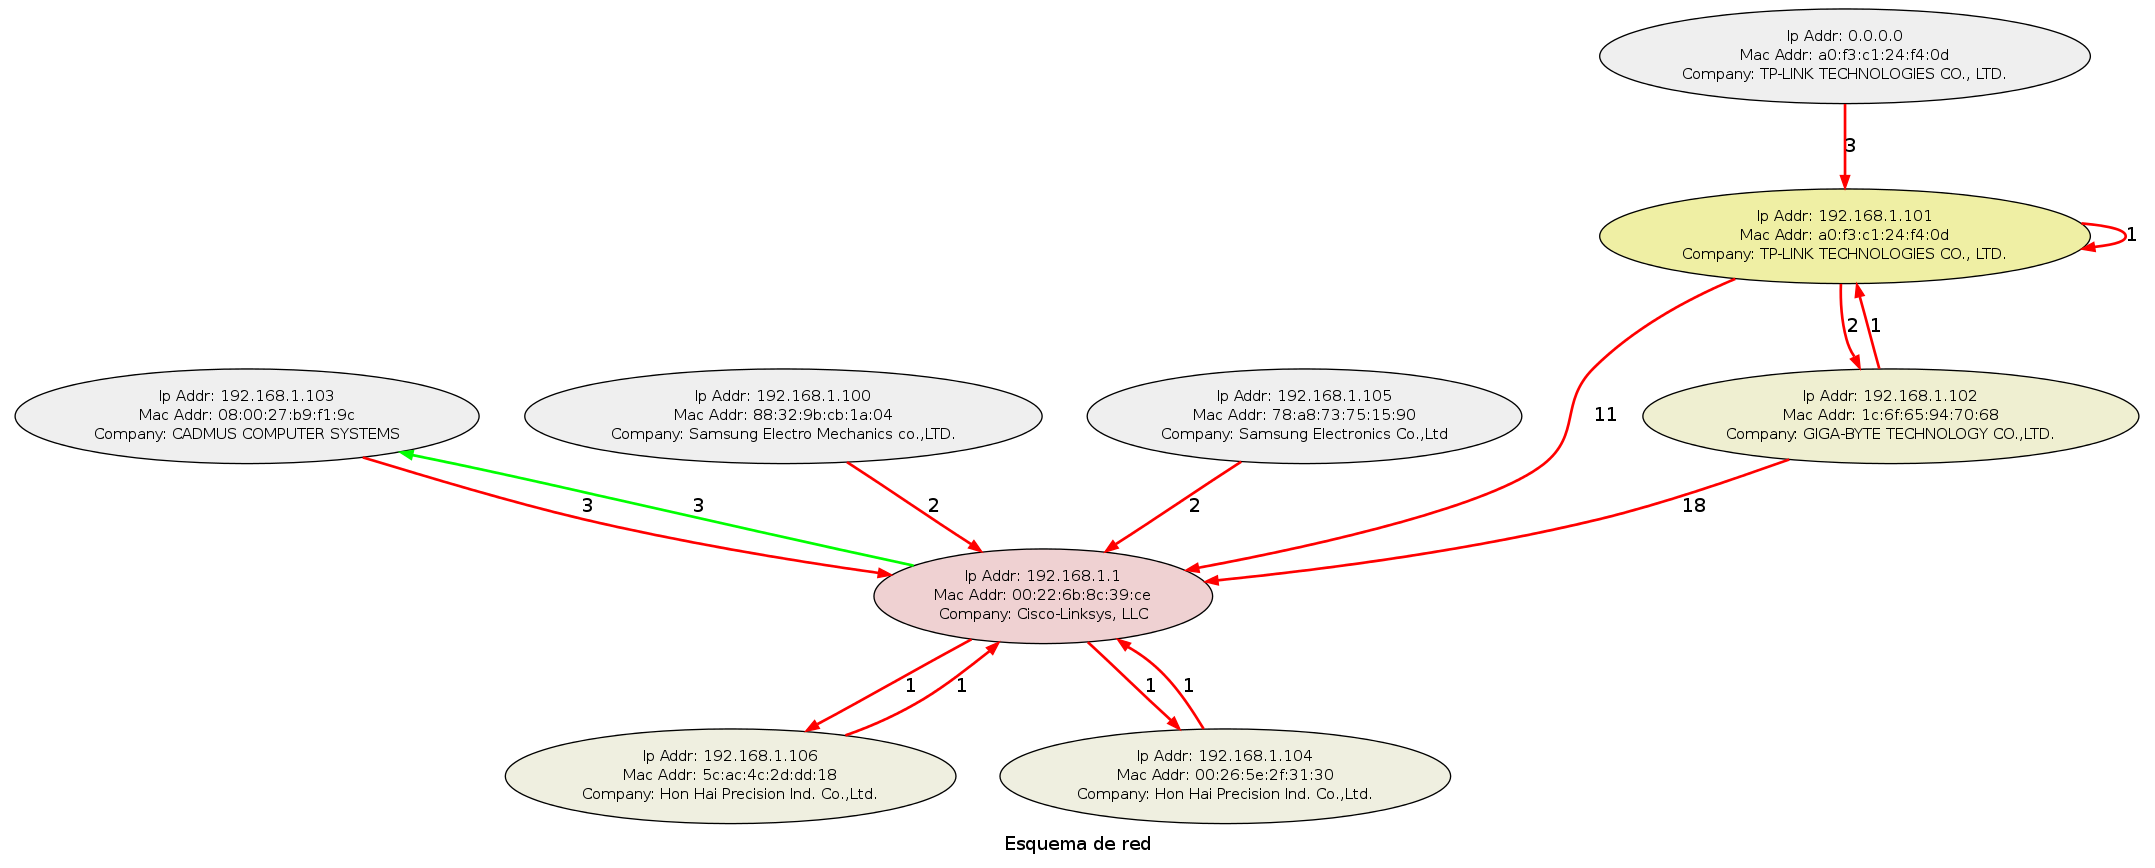
\includegraphics[scale=0.22]{../experimentacion-svilerino/casa/graph.png}
  \caption{Topologia de red estimada.}
\end{figure}


\subsubsection{Probabilidades y entropia de fuente origen}
\begin{figure}[h!]
  \centering
	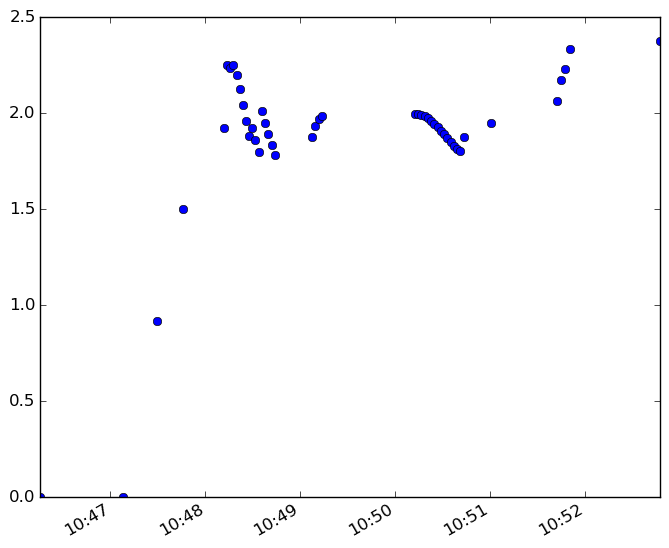
\includegraphics[scale=0.66]{../experimentacion-svilerino/casa/entropy_src.png}
  \caption{Entropia de la fuente origen.}
\end{figure}

\begin{figure}[h!]
  \centering
	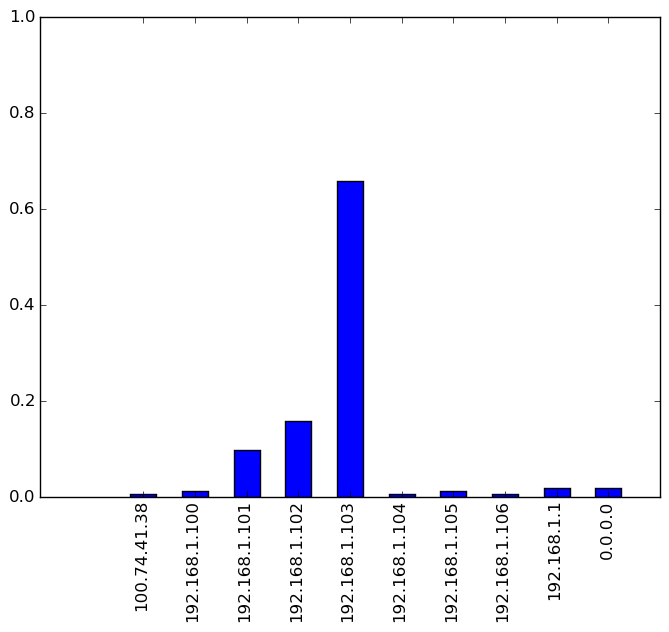
\includegraphics[scale=0.66]{../experimentacion-svilerino/casa/histogram_src_probabilities.png}
  \caption{Probabilidades asociadas a las IP de la fuente origen.}
\end{figure}

%---------------------------------------------------------------------------------------------------------------

\subsubsection{Probabilidades y entropia de fuente destino}
\begin{figure}[h!]
  \centering
	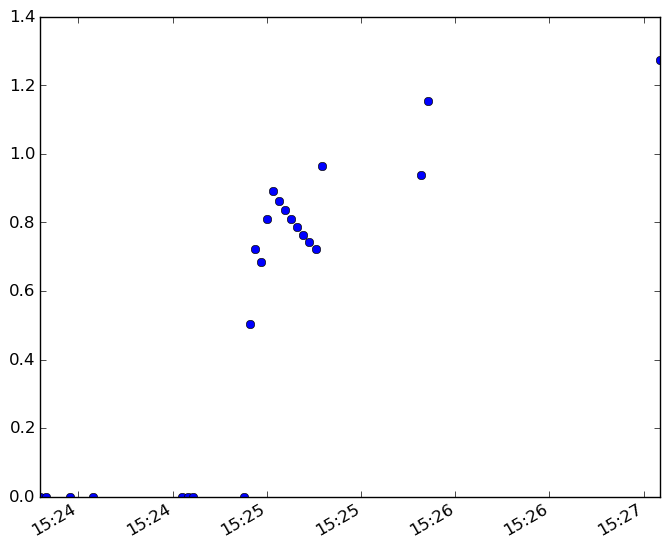
\includegraphics[scale=0.66]{../experimentacion-svilerino/casa/entropy_dst.png}
  \caption{Entropia de la fuente destino.}
\end{figure}

\begin{figure}[h!]
  \centering
	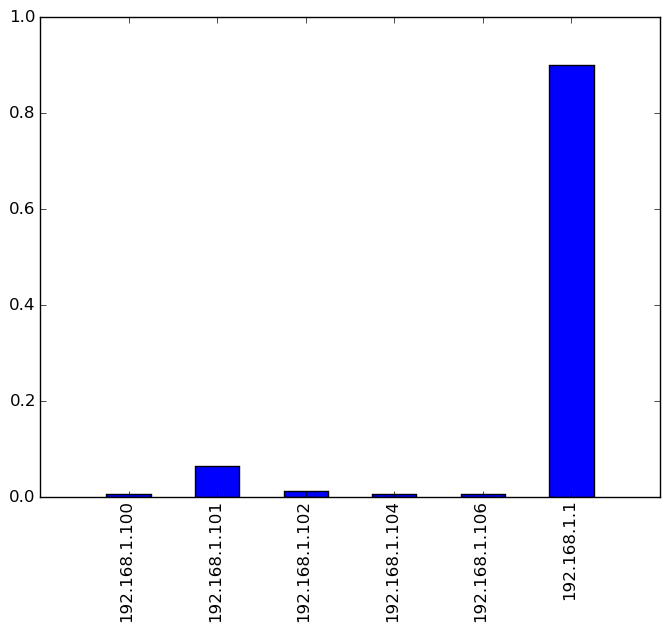
\includegraphics[scale=0.66]{../experimentacion-svilerino/casa/histogram_dst_probabilities.png}
  \caption{Probabilidades asociadas a las IP de la fuente destino.}
\end{figure}

\subsubsection{Tabla de dispositivos detectados}
\rowcolors{1}{Gray}{White}
\begin{tabular}{ |c|c|c| }
	\hline
	Ip Addr & Mac Addr & Company \\	
	\hline
	192.168.1.101 & a0:f3:c1:24:f4:0d & TP-LINK TECHNOLOGIES CO., LTD. \\
	\hline
	192.168.1.1 & 00:22:6b:8c:39:ce & Cisco-Linksys, LLC \\
	\hline
	100.74.41.38 & 88:32:9b:cb:1a:04 & Samsung Electro Mechanics co.,LTD. \\
	\hline
	192.168.1.105 & 78:a8:73:75:15:90 & Samsung Electronics Co.,Ltd \\
	\hline
	192.168.1.103 & 08:00:27:b9:f1:9c & CADMUS COMPUTER SYSTEMS \\
	\hline
	192.168.1.106 & 5c:ac:4c:2d:dd:18 & Hon Hai Precision Ind. Co.,Ltd. \\
	\hline
	192.168.1.102 & 1c:6f:65:94:70:68 & GIGA-BYTE TECHNOLOGY CO.,LTD. \\
	\hline
	192.168.1.104 & 00:26:5e:2f:31:30 & Hon Hai Precision Ind. Co.,Ltd. \\
	\hline
\end{tabular}

\subsubsection{Conclusiones del experimento}
Con respecto a los resultados obtenidos podemos inferir con cierta alta probabilidad que el nodo con IP \texttt{192.168.1.1} es el router de la red, tanto por el fabricante \texttt{Cisco-Linksys} como por la cantidad de pedidos who-has que preguntan por dicho nodo. El host 192.168.1.103 es el que realiza la escucha de la red por lo tanto tiene mas actividad que el resto de los nodos.